% \section{Experimental setup}
% One of the key parameter of the work is how we have used the dataset to create our train data to be able to correctly train our model.
% \par
% With LSTM and transformer model we could use the whole serie at one but it would not be very effective. For that, we have decided to use multiple sliding windows to create a dataset. The idea is to have an input window and a forecast window. There name are straigth forward everything in the input window is the input of the model and need to predict the forecast window. Figure~(\ref{fig:dataset_pretraitement}) represent this porcessus.

% \begin{figure}[H]
% \centering
% 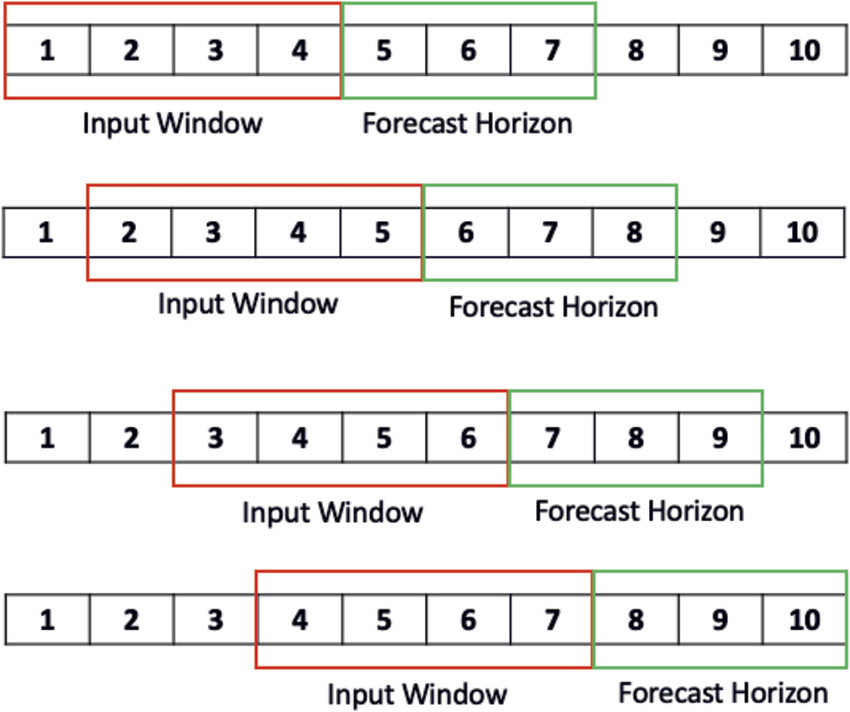
\includegraphics[width=0.6\textwidth]{images/dataset_pretraitement.jpg}
% \caption{Pretraitement of dataset to be used by our model}
% \label{fig:dataset_pretraitement}
% \end{figure}

% We made the input window of size 672 which represent a week of data and forecast for a period of 1 day which is 96 points. 
% \par
% This allow to train of shorter data more variate data at the expense that it impossible to learn relation in the data that is bigger than one week. We found this is okay because the data only evole on long period of time like a year and is most likely linked to something external on the client. There day to day consumption is pretty much similar every day and wanting to forecast those change on long term seams a bit surrealistic.
% \par
% This dataset also allow us to train the random forest regressor that will use this a vector of input and will create a vector of output. Without this, it would impossible to even forecast the anything.



% \par
% We apply this principe on the time series and them we split everything in 3 time series. The first one is used to train the model and take 80\% of the lenght. Then we have 10\% of validation followed by the last 10\% of for test. We have taken the data in the original serie in order above. It does not use random and so is always replicable.
% \par
% The idea is to get data to train model but for that we need verify our parameter with the dataset validation and after all we measure the performance with the test dataset.
% \par

% \par
% This seperation is not applyable on the ARIMA model. It want as input the whole time series. But we still perfomed the train, validation and test split.

% \par
% For the ARIMA model we used library \textit{pmdarima} which proposed a state of the art selection of the best parameter. For the Random Forest Regressor we used \textit{scikit-learn} which is also a state of the art implementation of this method. Those are pretty straitgh forward because they don't have a lot of parameter and trainer is already predone.

% \par
% For the RNN and transformer model, we have use \textit{TSAI} witch is a library that wrap above \textit{pytorch}. We have use the optimizer ADAM to optimize parameter and batch size to load multiple training element at once. 

% \par
% When we could decide the loss function we have used L1 loss function because it is more reliable when we have outlier and as seen in Figure~(\ref{fig:dataset}) we have some. 

% \par
% All our code is avaiable on our github \url{https://github.com/orbitalgamer/Advanced-Deep-Learning}.

\section{Experimental setup}

A key component of this work concerns how the dataset is structured and partitioned in order to train and evaluate the forecasting models in a consistent and reproducible manner.

\par
Although recurrent and transformer-based models are capable of processing long sequences, using the full time series as a single training example is neither efficient nor effective. Instead, we adopt a sliding-window approach to construct the training dataset. Each sample consists of an input window and a corresponding forecasting window. The input window is provided to the model, which is tasked with predicting the values in the forecast window. Figure~\ref{fig:dataset_pretraitement} illustrates this preprocessing procedure.

\begin{figure}[H]
\centering
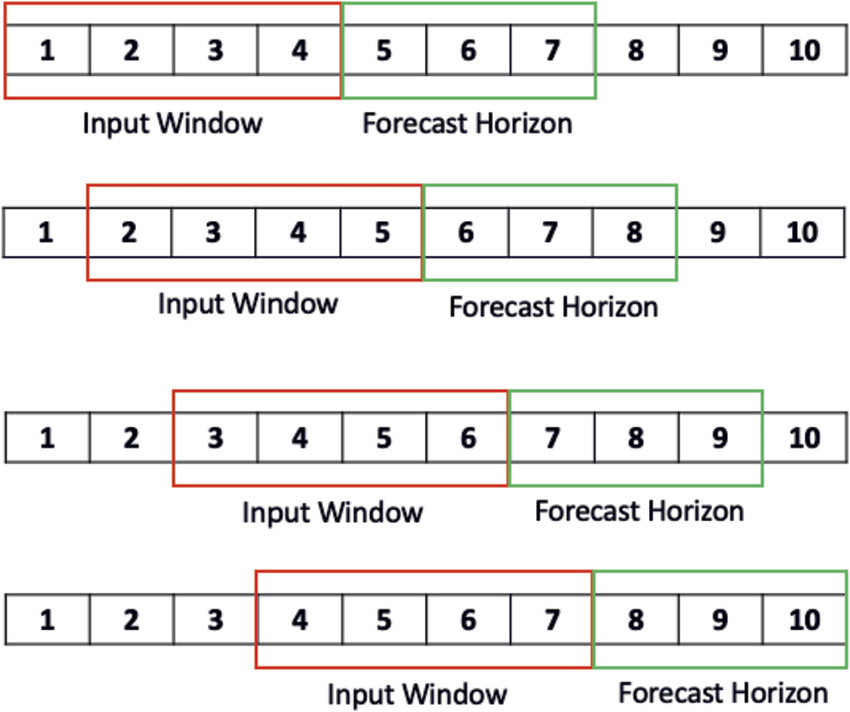
\includegraphics[width=0.6\textwidth]{images/dataset_pretraitement.jpg}
\caption{Sliding-window preprocessing applied to the time series}
\label{fig:dataset_pretraitement}
\end{figure}

\par
The input window length is set to 672 time steps, corresponding to one week of data, while the forecasting horizon is fixed to one day, i.e., 96 time steps. This configuration enables the generation of a large number of training samples from a single time series, thereby increasing data variability during training.

\par
This design choice limits the model’s ability to explicitly capture dependencies spanning more than one week. However, this constraint is considered acceptable in the present context, as long-term consumption trends (e.g., yearly variations) are likely driven by external factors specific to the client. In contrast, daily and weekly consumption patterns are relatively stable and therefore more amenable to short- and medium-term forecasting.

\par
The same sliding-window representation is also used to train the Random Forest Regressor, which requires fixed-size input and output vectors. Without this transformation, applying such a model to time series forecasting would not be feasible.

\par
After window generation, the data is split chronologically into three subsets: 80\% for training, 10\% for validation, and 10\% for testing. The split is performed in temporal order without random shuffling, ensuring that no future information is leaked into the training process and that all experiments are fully reproducible.

\par
The training set is used to fit model parameters, the validation set to tune hyperparameters, and the test set to evaluate final performance.

\par
This data partitioning strategy is not directly applicable to ARIMA-based models, which require a contiguous time series as input. Nevertheless, we retain the same temporal split and evaluate ARIMA forecasts on the validation and test segments in a consistent manner.

\par
For ARIMA modeling, we use the \textit{pmdarima} library, which provides automated and widely used procedures for selecting optimal model parameters. The Random Forest Regressor is implemented using \textit{scikit-learn}, which offers a well-established and efficient implementation with a limited number of tunable hyperparameters.

\par
Recurrent neural networks and transformer-based models are implemented using the \textit{tsai} library, which is built on top of \textit{PyTorch}. WE use \textit{TSTplus} model from \textit{tsai}. Model parameters are optimized using the Adam optimizer, and training is performed using mini-batches to improve computational efficiency.

\par
The L1 loss function is used for training neural network models, as it is more robust to outliers than the L2 loss. This choice is motivated by the presence of occasional high/low-consumption peaks in the dataset, as illustrated in Figure~\ref{fig:dataset}.

\par
All code and experimental configurations are publicly available at \url{https://github.com/orbitalgamer/Advanced-Deep-Learning}.


% \section{Experimental results}

% The first test we made was on forecasting only the next point. To avoidn recreating all model we forecast for the next 96 point and only take the first element. Which lead to the restult in Table~\ref{tab:1stepforecasting}


% \begin{table}[H]
%     \centering
%     \caption{Result of 1 step forecasting}
%     \label{tab:1stepforecasting}
    
    
%     \setlength{\tabcolsep}{6pt}
%     \renewcommand{\arraystretch}{1.1}
    
%     \begin{tabular}{l|c|c|c}
    
%     \hline
%     Method & MAE & MASE & SMAPE \\
%     \hline
%     ARIMA & 18,18     &1,04      &0,078        \\
%     \hline
%     Random Forest & 19,41     & 1,11      & 0,087        \\
%     \hline
%     LSTM & 16,53     & 0,95      &0,072        \\
%     \hline
%     Transformer & 14,55     & 0,8344      &0,063        \\
   
%     \hline
    
%     \end{tabular}
% \end{table}

% We observe here that ARIMA has result that are pretty good. But when we look at is graph on Figure~\ref{fig:arima_forecast} we observe that ARIMA just forecast the last know data point. Which is normal because with the size of data we were not able to put big parameter so that arima can look a lot of data in the past. Metric also look this good because we have a lot of point so we see that difference between an naive forecast and the actual consumption is small. 

% \begin{figure}[H]
% \centering
% 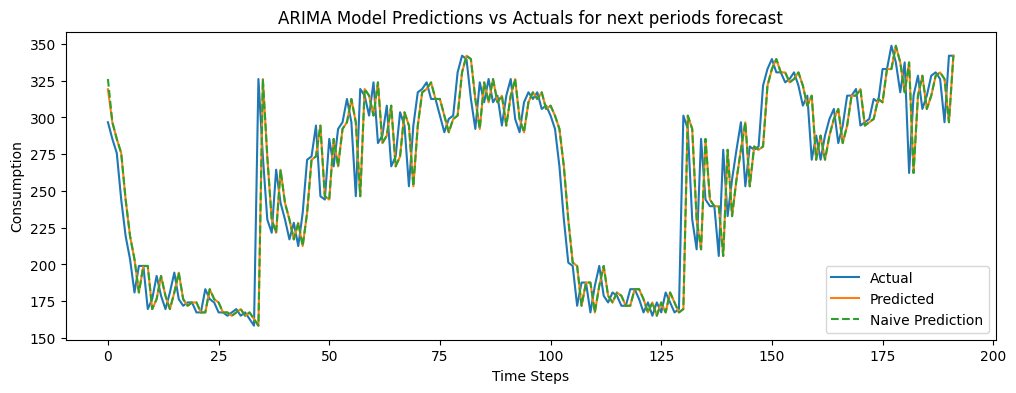
\includegraphics[width=1\textwidth]{images/arima.png}
% \caption{Forecasting of ARIMA method (for the 194 first points)}
% \label{fig:arima_forecast}
% \end{figure}

% For the rest of the result we observe that to forecast the next datapoint, transformer seems to outperform all the others. We also note that only LSTM and Transformer manage to get an MASE score tinir than 1 meaning they are better than just using a naive model which forecast all ways the last known data.

% The second test is on the forecast on a hole day. You can find the restult in the Table~\ref{tab:dayforecasting}.

% \begin{table}[H]
%     \centering
%     \caption{Result of 1 step forecasting}
%     \label{tab:dayforecasting}
    
    
%     \setlength{\tabcolsep}{6pt}
%     \renewcommand{\arraystretch}{1.1}
    
%     \begin{tabular}{l|c|c|c}
    
%     \hline
%     Method & MAE & MASE & SMAPE \\
%     \hline
%     ARIMA & 62,61     & 3,59      & 0,265        \\
%     \hline
%     Random Forest & 22,96     & 1,32      &0,102        \\
%     \hline
%     LSTM & 23,21     &1,33      &0,102        \\
%     \hline
%     Transformer & 23,86     &1,37      &0,107        \\
   
%     \hline
    
%     \end{tabular}
% \end{table}

% With these result we see that model have harder to forecast a day which is not suprising because we need to generate information later in time which could change potentialy a lot. We see that ARIMA is not able to forecast correctly. The few first step is okay and then is just an horizontal line which is realy bad.
% \par
% Now we don't see any paritcular trend if a model is better than another except for arima wich is horrible in comparaison to the 3 other. Random forest was the one that suffered the less from the greater window because it metric did not jump as much as the other models.
% \par
% Remark : MASE metric here I think does not mean anything because we forecast 96 point forward so a naive forecaster won't predict anything but by the definition that is computed on the training set. If we were to compute an MAE naive forecast on the test set we would have score that are close to the MAE value which would lead to have MASE score coser to 0,37 which is significantly better.


\section{Experimental results}

The first experiment evaluates one-step-ahead forecasting performance. In order to avoid retraining separate models, each model is configured to predict the next 96 time steps, and only the first predicted value is retained for evaluation. The resulting performance metrics are reported in Table~\ref{tab:1stepforecasting}.

\begin{table}[H]
    \centering
    \caption{Results of one-step-ahead forecasting}
    \label{tab:1stepforecasting}
    \setlength{\tabcolsep}{6pt}
    \renewcommand{\arraystretch}{1.1}
    \begin{tabular}{l|c|c|c}
    \hline
    Method & MAE & MASE & SMAPE \\
    \hline
    ARIMA & 18.18 & 1.04 & 0.078 \\
    Random Forest & 19.41 & 1.11 & 0.087 \\
    LSTM & 16.53 & 0.95 & 0.072 \\
    Transformer & 14.55 & 0.83 & 0.063 \\
    \hline
    \end{tabular}
\end{table}

\par
ARIMA achieves relatively competitive error metrics in this setting. However, inspection of its forecasts (Figure~\ref{fig:arima_forecast}) reveals that the model  predicts values close to the last observed data point. This behavior is consistent with the limited autoregressive order used, which was constrained by the length of the training window. In addition, the small error magnitude can be partially explained by the high sampling frequency of the data, where consecutive observations tend to be similar, making naive or near-naive forecasts appear effective under one-step evaluation metrics.

\begin{figure}[H]
\centering
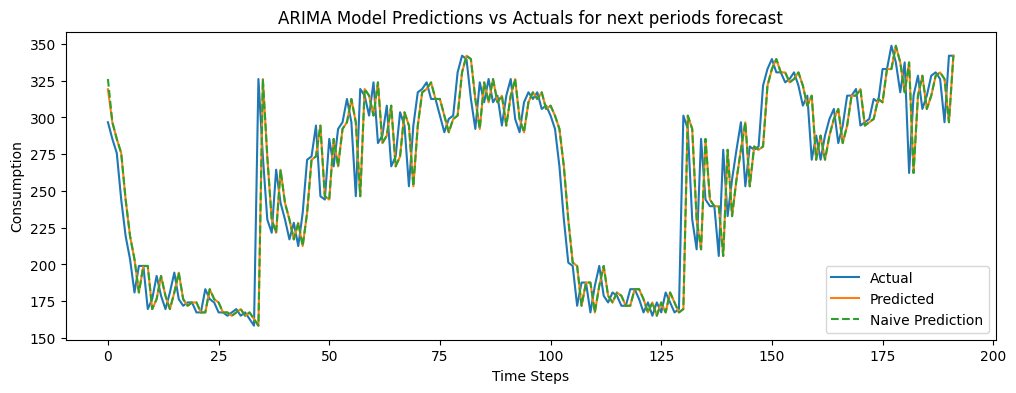
\includegraphics[width=1\textwidth]{images/arima.png}
\caption{One-step-ahead forecasting using the ARIMA model (first 194 points)}
\label{fig:arima_forecast}
\end{figure}

\par
Among the remaining models, the transformer achieves the best overall performance for one-step-ahead forecasting across all metrics. Notably, only the LSTM and transformer models obtain MASE values below 1, indicating performance superior to a naive persistence baseline.

\par
The second experiment evaluates multi-step forecasting over a full day (96 time steps). The corresponding results are presented in Table~\ref{tab:dayforecasting}.

\begin{table}[H]
    \centering
    \caption{Results of one-day-ahead forecasting}
    \label{tab:dayforecasting}
    \setlength{\tabcolsep}{6pt}
    \renewcommand{\arraystretch}{1.1}
    \begin{tabular}{l|c|c|c}
    \hline
    Method & MAE & MASE & SMAPE \\
    \hline
    ARIMA & 62.61 & 3.59 & 0.265 \\
    Random Forest & 22.96 & 1.32 & 0.102 \\
    LSTM & 23.21 & 1.33 & 0.102 \\
    Transformer & 23.86 & 1.37 & 0.107 \\
    \hline
    \end{tabular}
\end{table}

\par
As expected, forecasting performance degrades for all models when predicting a full day ahead, reflecting the increased uncertainty associated with longer forecasting horizons. The ARIMA model performs particularly poorly in this setting, as errors accumulate rapidly during recursive multi-step prediction. While the initial forecasted steps are reasonable, the model quickly converges to constant predictions, resulting in large overall errors.

\par
Among the remaining approaches, no single model clearly dominates across all metrics. However, the Random Forest Regressor exhibits the smallest relative degradation in performance when transitioning from one-step to one-day forecasting, suggesting greater robustness to increasing prediction horizons in this experimental setup.

\par
% It is worth noting that the interpretation of the MASE metric in the multi-step forecasting setting is less straightforward. Since MASE is normalized using the error of a one-step-ahead naive model computed on the training set. The idea behind this metric is to see if the model is better than a naive forecaster. So if we apply a naive forecaster on this test dat while only knowing the first element, it will just predict this element over and over which would yield to an MAE score way higher that would led to MASE way smaller. As shown before, the ARIMA is not realy far from the naive forcast and has an MAE of 62,61. With that in mind we can say that MASE for other model should be around 0,35-0,40 which is considerably better.







% Now for the long term forecasting, you can find all the restult in the Figure~\ref{fig:maelongtermforecast},\ref{fig:maselongtermforecast} and \ref{fig:smapelongtermforecast}. You can see in those graphs that the metric quickly rise up which mean that we have error accumulating. As shown before our model are not perfect to generate the data for a day and now we reuse this data thus making a lot of error accumulation.



% \begin{figure}[H]
% \centering
% 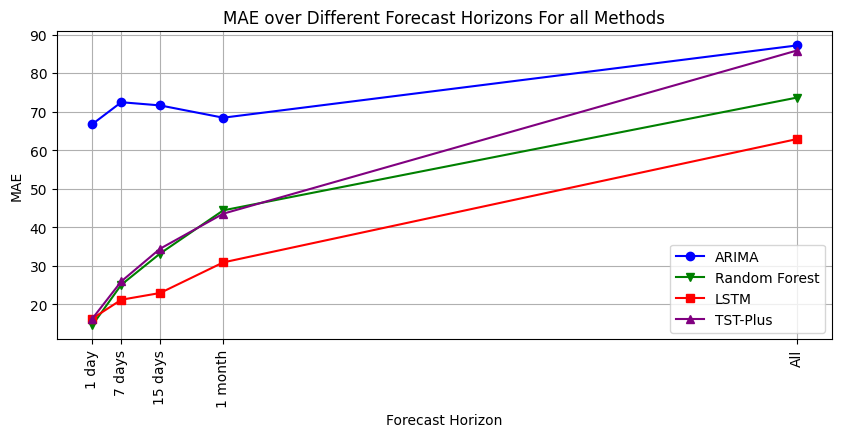
\includegraphics[width=1\textwidth]{images/MAE_longterm_forecasting.png}
% \caption{Evolution of MAE for different forecasating periode for each model}
% \label{fig:maelongtermforecast}
% \end{figure}

% \begin{figure}[H]
% \centering
% 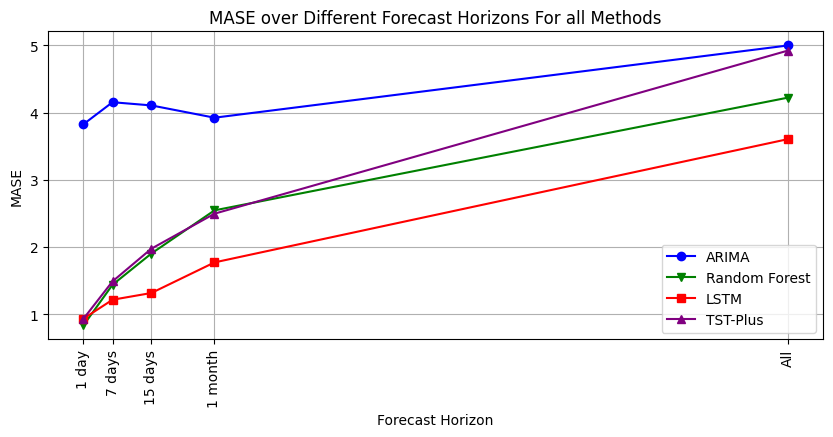
\includegraphics[width=1\textwidth]{images/MASE_longterm_forecasting.png}
% \caption{Evolution of MASE for different forecasating periode for each model}
% \label{fig:maselongtermforecast}
% \end{figure}

% \begin{figure}[H]
% \centering
% 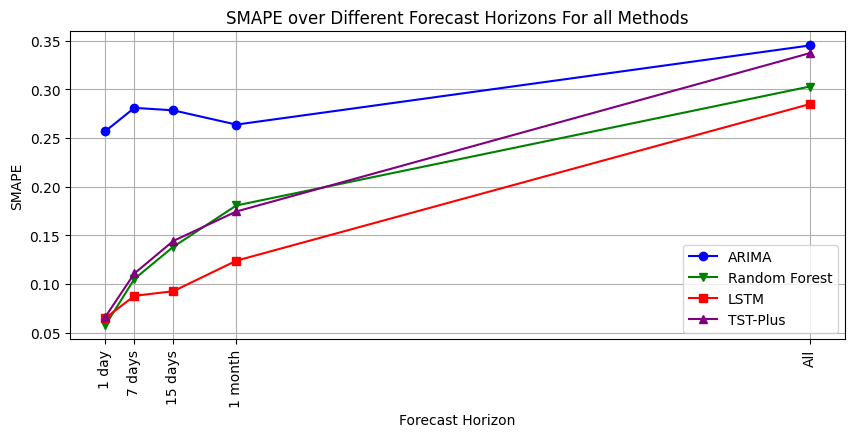
\includegraphics[width=1\textwidth]{images/SMAPE_longterm_forecasting.png}
% \caption{Evolution of SMAPE for different forecasating periode for each model}
% \label{fig:smapelongtermforecast}
% \end{figure}
% \par
% On all this model, LSTM appear to be better than all other model for long term forecasting with this mecanisme of recusrive forecasting. But in aboslute those metrics are okay until days 15 of forecasting. It is said that SMAPE metric under 10\% are considered higly accurate, and up to 20\% is considered somewhat accurate\cite{Makridakis2000-ml}. The Figure~\ref{fig:lstmlongterm} show the forecast for the first 30 day. Eventhough metric says it could be okay ot use up to 30 days we would not forecast for period greater than 15 days.


% \begin{figure}[H]
% \centering
% 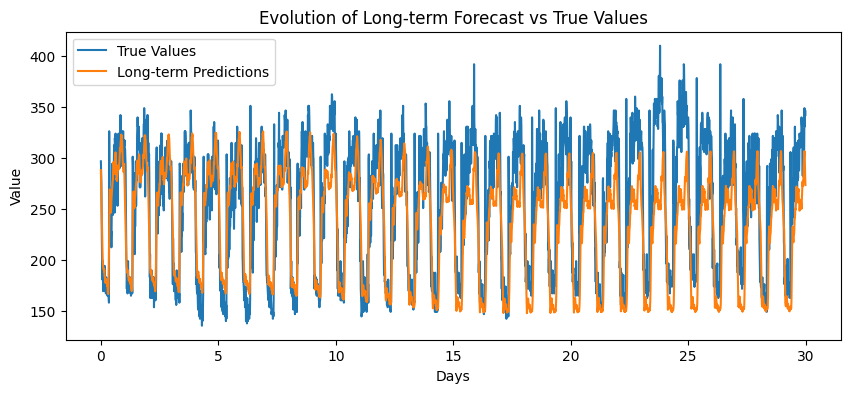
\includegraphics[width=1\textwidth]{images/lstm.png}
% \caption{Evolution of Long-term Forecast in comparaison to true value}
% \label{fig:lstmlongterm}
% \end{figure}

It is important to note that the interpretation of the MASE metric becomes less straightforward in a multi-step forecasting setting. By definition, MASE is normalized using the error of a one-step-ahead naive forecasting model computed on the training set. The primary purpose of this metric is to assess whether a forecasting model outperforms a simple persistence baseline.

\par
In the context of long-horizon forecasting, this normalization can be misleading. If a naive forecaster is applied to the test set while only observing the first value of the forecasting horizon, it will repeatedly predict this value for all subsequent time steps. Such behavior would result in a substantially larger MAE over a 96-step horizon, and consequently yield much smaller MASE values when used as a normalization baseline.

\par
As discussed previously, the ARIMA model produces forecasts that are close to a naive persistence strategy and achieves an MAE of 62.61 for one-day-ahead forecasting. Under this perspective, the effective MASE values for the remaining models would be expected to lie approximately in the range of 0.35 to 0.40, indicating significantly better performance relative to a naive multi-step baseline.

\par
Long-term forecasting performance is illustrated in Figures~\ref{fig:maelongtermforecast}, \ref{fig:maselongtermforecast}, and \ref{fig:smapelongtermforecast}. These figures show a rapid increase in error metrics as the forecasting horizon grows, highlighting the accumulation of prediction errors inherent to recursive forecasting strategies. Since predicted values are reused as inputs for subsequent predictions, even small inaccuracies can compound over time.

\begin{figure}[H]
\centering
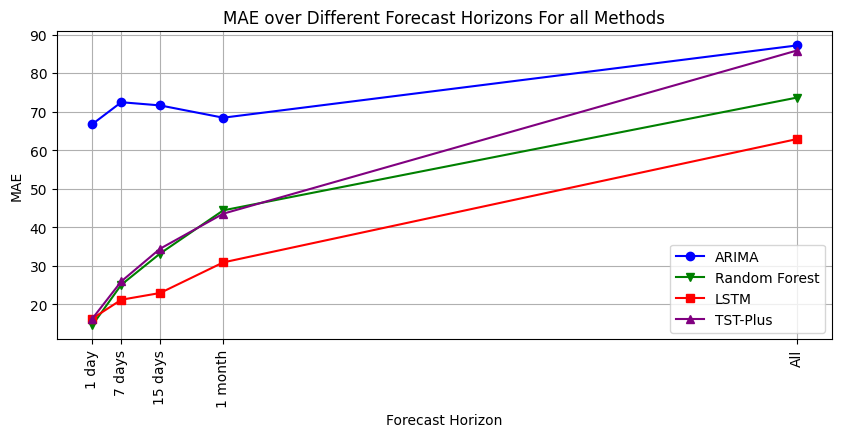
\includegraphics[width=0.85\textwidth]{images/MAE_longterm_forecasting.png}
\caption{Evolution of MAE across different forecasting horizons for each model}
\label{fig:maelongtermforecast}
\end{figure}

\begin{figure}[H]
\centering
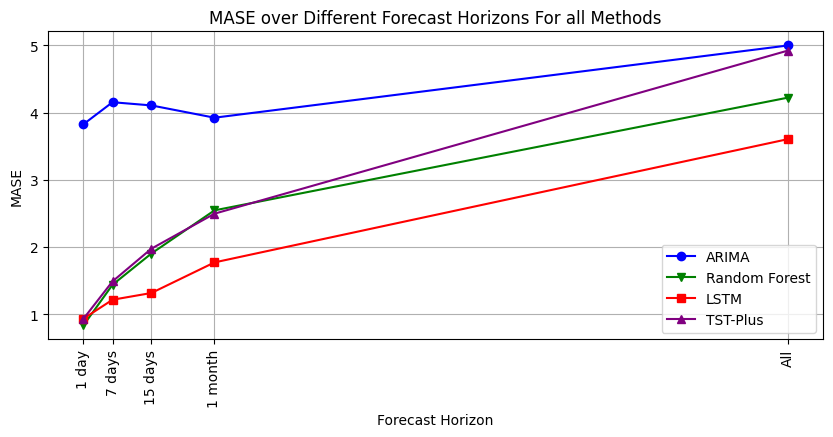
\includegraphics[width=0.85\textwidth]{images/MASE_longterm_forecasting.png}
\caption{Evolution of MASE across different forecasting horizons for each model}
\label{fig:maselongtermforecast}
\end{figure}

\begin{figure}[H]
\centering
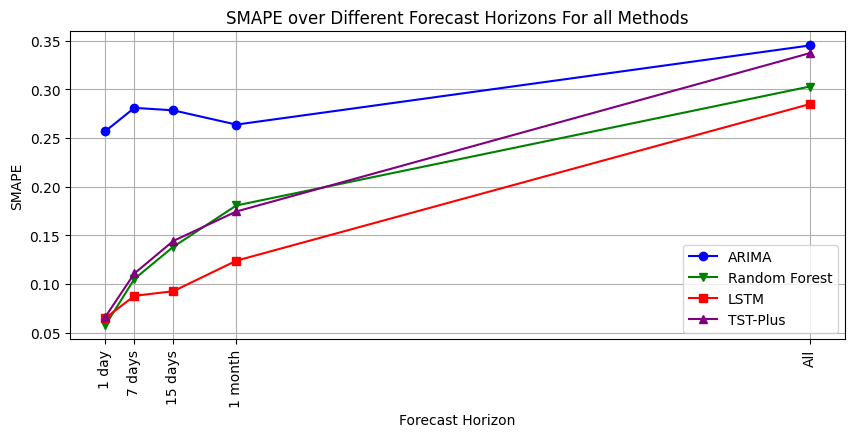
\includegraphics[width=0.85\textwidth]{images/SMAPE_longterm_forecasting.png}
\caption{Evolution of SMAPE across different forecasting horizons for each model}
\label{fig:smapelongtermforecast}
\end{figure}

\par
Among all evaluated models, the LSTM consistently demonstrates superior robustness for long-term forecasting under a recursive prediction scheme. Nevertheless, absolute performance metrics remain within acceptable ranges only up to approximately 30 days ahead. According to commonly used interpretative guidelines, SMAPE values below 10\% are considered highly accurate, while values up to 20\% are regarded as moderately accurate \cite{Makridakis2000-ml}.

\par
Figure~\ref{fig:lstmlongterm} presents the LSTM forecast over the first 30 days. Although the error metrics suggest that predictions may remain usable beyond 15 days, we would conservatively limit the practical forecasting horizon to two weeks, beyond which uncertainty becomes increasingly pronounced.

\begin{figure}[H]
\centering
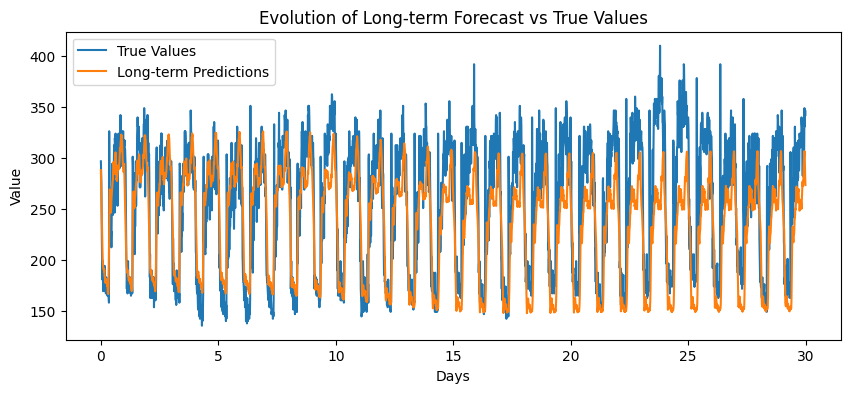
\includegraphics[width=0.9\textwidth]{images/lstm.png}
\caption{Long-term LSTM forecasts compared to ground truth}
\label{fig:lstmlongterm}
\end{figure}
